El uso de los m\'etodos de PCA y PLS-DA se funda en reducir la dimensi\'on de los datos a clasificar. La idea es capturar la mayor cantidad de informaci\'on, dejando de lado las componentes que en determinado momento dejen de ofrecernos datos relevantes.

Para esto proponemos el siguiente m\'etodo: Tomamos toda la base de entrenamiento, dejando vac\'ia la base de \textit{test}, y calculamos los 784 autovalores para ambos m\'etodos. Sea $\lambda_{PCA}$ la suma de los autovalores obtenidos por PCA y $\lambda_{PLS-DA}$ la suma de los obtenidos por PLS-DA.

En el caso de PCA, como siempre calculamos los autovalores de la matriz de covarianzas, se cumple que la suma de los autovalores es igual a la suma de las varianzas, es decir, a traza de la matriz de covarianzas. Entonces podemos decir que $\lambda_{PCA}^{i} / \lambda_{PCA}$ representa el porcentaje de varianza que absorbe el $i$-\'esimo autovalor.

Si acumulamos las varianzas que absorbe cada vector, se genera el siguiente gr\'afico:

\begin{figure}[h!]
  \begin{center}
	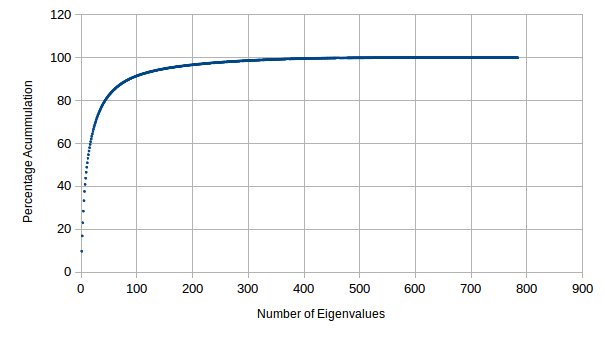
\includegraphics[scale=1]{exp4/PCA-percentage.png}
	\caption{Porcentaje de varianzas acumuladas: PCA}
	\label{accum_var_PCA}
  \end{center}
\end{figure}

Puede verse que el primer autovector se lleva el 10\% de la varianza, el segundo casi un 7\%. Pero es m\'as interesante cuando se llega a tomar 50 autovalores, en esta caso, ya se tom\'o cerca de 83\% de la informaci\'on. Con lo cual, podr\'iamos pensar los dem\'as autovalores no son tan significativos \footnote{El 90\% se alcanza con 86 autovalores. El 99\% con 330}.

Para el caso de PLS-DA, no se calculan los autovalores de la misma matriz en cada paso, haciendo que el an\'alisis anterior no sea del todo directo. Notemos que el autovalor obtenido en cada paso, si bien es de una matriz diferente, tiene la idea de maximimar las varianzas y minimizar las covarianzas de la uni\'on entre las im\'agenes y sus etiquetas. Entonces decidimos aplicar el mismo procedimiento, obteniendo estos resultados:

\newpage

\begin{figure}[h!]
  \begin{center}
	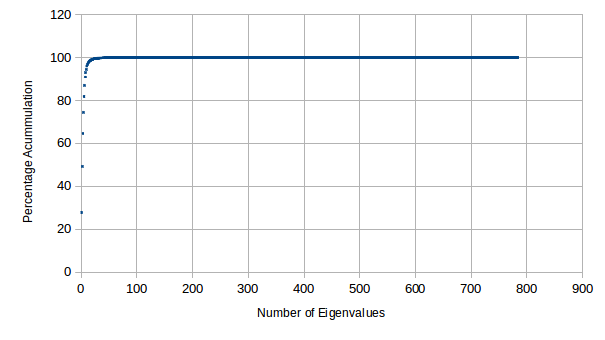
\includegraphics[scale=1]{exp4/PLSDA-percentage.png}
	\caption{Porcentaje de varianzas acumuladas: PLS-DA}
	\label{accum_var_PLSDA}
  \end{center}
\end{figure}

En este se ve que ya el primer autovector, captura cerca del 30\% de la informaci\'on. Junto al segundo, consumen casi el 50\%. Esto indica que tener en cuenta la etiqueta a la hora de intentar reducir la dimensi\'on de los datos puede ser muy \'util. De hecho, con 8 autovalores se captura el 90\% y con 18 ya el 99\%

Los subsiguientes an\'alisis cualitativos fueron realizados bajo estas conclusiones. Es decir, no consideramos tomar $\alpha$ mayor a 300 ni $\gamma$ mayor a 20.
